\documentclass[aspectratio=169]{beamer}
\usetheme{Madrid}
\usepackage{amsmath,amssymb,graphicx}
\usepackage{booktabs}
\usepackage{hyperref}
\usepackage{tikz}

\def\b{\begin{equation}}
\def\e{\end{equation}}

% 4x4 Ising lattice: #1 = x offset, #2 = 16 spins (row by row), #3 = highlighted site
\newcommand{\isinglattice}[3]{%
  \begin{scope}[xshift=#1cm]
    \foreach \p in {0,...,3} {
      \draw[gray!60] (-0.35,\p*0.7) -- (2.45,\p*0.7);
      \draw[gray!60] (\p*0.7,-0.35) -- (\p*0.7,2.45);
    }
    \foreach \sp [count=\k from 0] in {#2} {
      \pgfmathtruncatemacro{\col}{mod(\k,4)}
      \pgfmathtruncatemacro{\row}{3-int(\k/4)}
      \ifnum\k=#3
        \fill[orange!45] (\col*0.7,\row*0.7) circle (0.31);
      \fi
      \ifnum\sp>0
        \draw[-latex,very thick,blue!75!black]
          (\col*0.7,\row*0.7-0.22) -- (\col*0.7,\row*0.7+0.22);
      \else
        \draw[-latex,very thick,red!75!black]
          (\col*0.7,\row*0.7+0.22) -- (\col*0.7,\row*0.7-0.22);
      \fi
    }
  \end{scope}%
}

\title[Discrete PIK]{Discrete Physics-Informed Kernels}
\author{Linus Gerlach}
\institute[ITP Heidelberg]{ITP Heidelberg}
\date{\today}

\begin{document}

\begin{frame}
  \titlepage
\end{frame}

\section{Motivation}

\begin{frame}{Path integrals and the Ising model}
  Euclidean lattice QFTs and statistical systems share the same observables:
  \b
    \langle O \rangle = \int \prod_{x\in\Lambda} d\phi_x\; O(\phi)\, e^{-\hat{S}(\phi)},
    \qquad \hat{S}(\phi) = S(\phi) + \ln\mathcal N,
    \qquad \mathcal N = \int \prod_{x\in\Lambda} d\phi_x\; e^{-S(\phi)} .
  \e
  \begin{columns}[c]
    \begin{column}{0.46\textwidth}
      \textbf{Ising model:} spins $s_x=\pm1$, with
      \b
        S(s) = \beta H(s) = -\beta\sum_{\langle x,y\rangle} s_x s_y .
      \e
      \begin{itemize}
        \item Phase transition at $\beta_c\approx 0.4407$
        \item $2^V$ states: no exact sums
        \item $s^{(i)}$: spin $i$ flipped
      \end{itemize}
    \end{column}
    \begin{column}{0.52\textwidth}
      \centering
      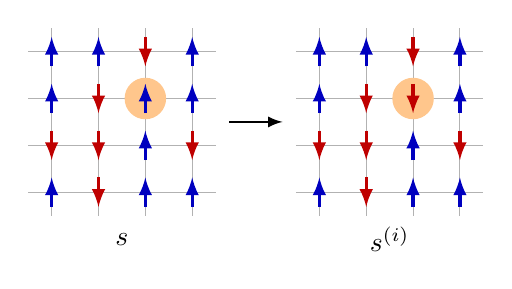
\begin{tikzpicture}[scale=0.85]
        \isinglattice{0}{1,1,-1,1,1,-1,1,1,-1,-1,1,-1,1,-1,1,1}{6}
        \isinglattice{4}{1,1,-1,1,1,-1,-1,1,-1,-1,1,-1,1,-1,1,1}{6}
        \draw[-latex,thick] (2.65,1.05) -- (3.45,1.05);
        \node at (1.05,-0.7) {$s$};
        \node at (5.05,-0.7) {$s^{(i)}$};
      \end{tikzpicture}
    \end{column}
  \end{columns}
  \vspace{0.4em}
  \begin{center}
    \textbf{So we want to sample from $p=e^{-S}/\mathcal N$.}
  \end{center}
\end{frame}

\begin{frame}{Monte Carlo and critical slowing down}
  \textbf{Importance sampling.} Draw $\phi^{(1)},\dots,\phi^{(N)} \sim p$ and estimate
  \b
    \langle O \rangle \approx \bar O_N = \frac{1}{N}\sum_{k=1}^{N} O(\phi^{(k)}),
    \qquad
    \sigma_{\bar O_N}^2 \approx \frac{2\tau_{\rm int}}{N}\,\mathrm{Var}(O) .
  \e

  \textbf{Markov chain Monte Carlo.} Generate samples with a kernel $T$ obeying detailed balance,
  \b
    p(\phi)\, T(\phi\to\phi') = p(\phi')\, T(\phi'\to\phi),
  \e
  e.g.\ Metropolis: propose $\phi\to\phi'$, accept with prob.\ $\min\bigl(1, e^{-\Delta S}\bigr)$.

  \vspace{0.3em}
  \begin{alertblock}{Critical slowing down}
    At $\beta_c$, local updates must relax over diverging correlations:
    $\tau_{\rm int}\propto\xi^z\propto L^z$, with $z\approx 2.17$.
    Cluster algorithms help the ferromagnet, but do not generalise to frustrated systems.
  \end{alertblock}
\end{frame}

\section{Method}

\begin{frame}{Physics-informed kernels: transport $p_0$ to $p_1$}
  \begin{center}
    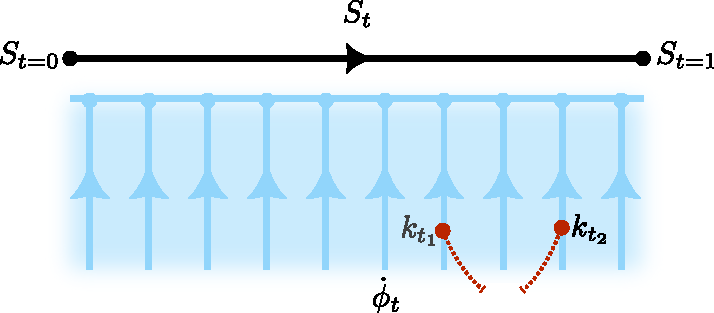
\includegraphics[width=0.46\textwidth]{figures/PIKConceptual.pdf}
  \end{center}
  \begin{columns}[t]
    \begin{column}{0.46\textwidth}
      \begin{block}{$p_0=e^{-S_0}/\mathcal N_0$: easy to sample}
        High temperature, $\beta_0<\beta_c$
      \end{block}
    \end{column}
    \begin{column}{0.46\textwidth}
      \begin{alertblock}{$p_1=e^{-S_1}/\mathcal N_1$: hard to sample}
        Phase transition, $\beta_1=\beta_c$
      \end{alertblock}
    \end{column}
  \end{columns}
  \begin{itemize}
    \item The kernel $\dot\phi_t$ moves samples along $p_t=e^{-S_t}/\mathcal N_t$, $S_t=\beta_t H$: no
      equilibration at $\beta_c$.
    \item Spins $s\in\{\pm1\}^V$ have no vector field $\dot\phi_t$: replace it by a Markov
      jump generator $Q_t$.
  \end{itemize}
\end{frame}

\begin{frame}{Discrete PIKs: the Kolmogorov equation}
  Samples move by spin flips with rates $Q_t\ge0$ (non-equilibrium, no detailed balance):
  \b
    \dot p_t(s) = \sum_{i}\underbrace{\Bigl[p_t(s^{(i)})\,Q_t(s^{(i)},s) - p_t(s)\,Q_t(s,s^{(i)})\Bigr]}_{-J_i(s)} .
  \e
  To carry $p_0$ to $p_1$ along $p_t=e^{-S_t}/\mathcal N_t$, the left-hand side is prescribed:
  \b
    \dot p_t(s) = \dot\beta_t\, p_t(s)\bigl(\langle H\rangle_t - H(s)\bigr) .
  \e
  \textbf{Minimal split.} Only the net current $J_i$ is constrained; the smallest non-negative
  rates are
  \b
    Q_t(s,s^{(i)}) = \frac{\max\bigl(J_i(s),0\bigr)}{p_t(s)} .
  \e
\end{frame}

\begin{frame}{Discrete PIKs: the graph Poisson equation}
  The constraint leaves $J$ undetermined (the hypercube of configurations has cycles).
  Select the least dissipative current:
  \b
    \min_J\ \frac12\sum_{\rm edges}\frac{J^2}{\chi},
    \qquad \chi_i(s) = \frac{p_t(s)-p_t(s^{(i)})}{\ln p_t(s)-\ln p_t(s^{(i)})} .
  \e
  The minimiser is a gradient, $J_i(s)=\chi_i(s)\bigl(\Phi_t(s)-\Phi_t(s^{(i)})\bigr)$, which gives
  \b
    (L_t\Phi_t)(s) = \sum_i \chi_i(s)\bigl(\Phi_t(s)-\Phi_t(s^{(i)})\bigr) = -\dot p_t(s) .
  \e
  \begin{itemize}
    \item Solve for $\Phi_t$, read off $J_i$, then $Q_t$.
    \item Independent walkers from $p_0$ stay exactly on $p_t$: no waiting time $\tau$ at $\beta_c$.
  \end{itemize}
\end{frame}

\section{Optimal transport}

\begin{frame}{Optimal transport: the minimal-dissipation schedule}
  \begin{columns}[c]
    \begin{column}{0.56\textwidth}
      Which path $\beta_t$ from $p_0$ to $p_1$ is best? Since $\Phi_t=\dot\beta_t\,\psi_{\beta_t}$,
      the dissipation (Maas 2011) is a length functional:
      \b
        \mathcal A[\beta] = \int_0^1 D(\beta_t)\,\dot\beta_t^2\,dt,
        \qquad D(\beta)=\psi_\beta^T L_\beta\,\psi_\beta .
      \e
      With $\ell(\beta)=\int_{\beta_0}^{\beta}\sqrt{D(b)}\,db$, Cauchy--Schwarz gives
      $\mathcal A\ge\ell(\beta_1)^2$, saturated by the geodesic
      \b
        \beta^*(t) = \ell^{-1}\bigl(t\,\ell(\beta_1)\bigr).
      \e
    \end{column}
    \begin{column}{0.42\textwidth}
      \centering
      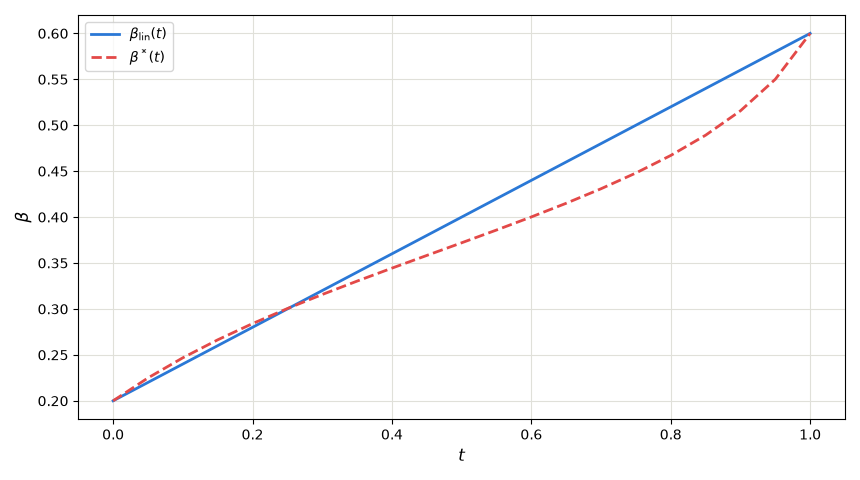
\includegraphics[width=\textwidth]{figures/schedule_comparison.png}
    \end{column}
  \end{columns}
  \vspace{0.4em}
  \begin{itemize}
    \item $4\times4$ lattice: $D(\beta)$ peaks at $\beta\approx0.37$; $\mathcal A$ only falls
      from $6.68$ to $5.96$.
    \item Fixed-step tracking gets worse ($1.25\times10^{-6}\to4.8\times10^{-3}$): the late
      speed-up of $\beta^*$ produces a burst of large rates.
  \end{itemize}
\end{frame}

\section{Outlook}

\begin{frame}{Outlook: causal dynamical triangulations}
  CDT is a path integral of the same form, over triangulations $T$ instead of spins:
  \b
    Z(\kappa) = \sum_{T}\frac{1}{C_T}\,e^{-S(T;\kappa)},
    \qquad S(T;\kappa) = \sum_a \kappa_a N_a(T) .
  \e
  \begin{columns}[c]
    \begin{column}{0.66\textwidth}
      \begin{itemize}
        \item Couplings $\kappa$ replace $\beta$, local moves replace spin flips.
        \item Kolmogorov and Poisson equations carry over formally.
        \item No enumeration at physical sizes: approximations are needed.
        \item First test: 1+1D CDT, which is exactly solvable.
      \end{itemize}
    \end{column}
    \begin{column}{0.32\textwidth}
      \centering
      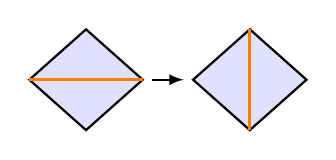
\begin{tikzpicture}[scale=0.8]
        \foreach \dx/\a/\b in {0/0/2,2.6/1/3} {
          \coordinate (P0) at (\dx+0,0.8);
          \coordinate (P1) at (\dx+0.9,0);
          \coordinate (P2) at (\dx+1.8,0.8);
          \coordinate (P3) at (\dx+0.9,1.6);
          \fill[blue!12] (P0)--(P1)--(P2)--(P3)--cycle;
          \draw[thick] (P0)--(P1)--(P2)--(P3)--cycle;
          \draw[very thick,orange] (P\a)--(P\b);
        }
        \draw[-latex,thick] (1.95,0.8) -- (2.45,0.8);
      \end{tikzpicture}

      \vspace{0.2em}
      \scriptsize $(2,2)$ move: the analogue of a spin flip
    \end{column}
  \end{columns}
\end{frame}

\end{document}
